\documentclass[11pt,a4paper,twocolumn, bold]{report}

\usepackage[left=2cm,right=2cm,top=1.75cm,bottom=1.75cm,columnsep=0.75cm]{geometry}
\usepackage[document]{ragged2e} 
\usepackage[pages=some]{background}
\usepackage{titling}
\usepackage{fancyhdr} 
\usepackage{titlesec}
\usepackage{etoolbox}
\usepackage{pdflscape}
\usepackage{incgraph,tikz}

\makeatletter
\patchcmd{\scr@startchapter}{\if@openright\cleardoublepage\else\clearpage\fi}{}{}{}
\makeatother


\title{}
\date{}

\fancyhf{}
\cfoot{\thepage}
\pagestyle{fancy}

%\titleformat{\chapter}[display]{\normalfont\bfseries}{}{0pt}{\Large}
\titleformat*{\section}{\LARGE\bfseries}
\titlespacing{\section}{-5pt}{5pt}{5pt}

\titlespacing{\subsection}{0pt}{5pt}{5pt}

\renewcommand{\thesection}{\arabic{section}}


\backgroundsetup{
scale=1,
color=black,
opacity=0.6,
angle=0,
contents={%
  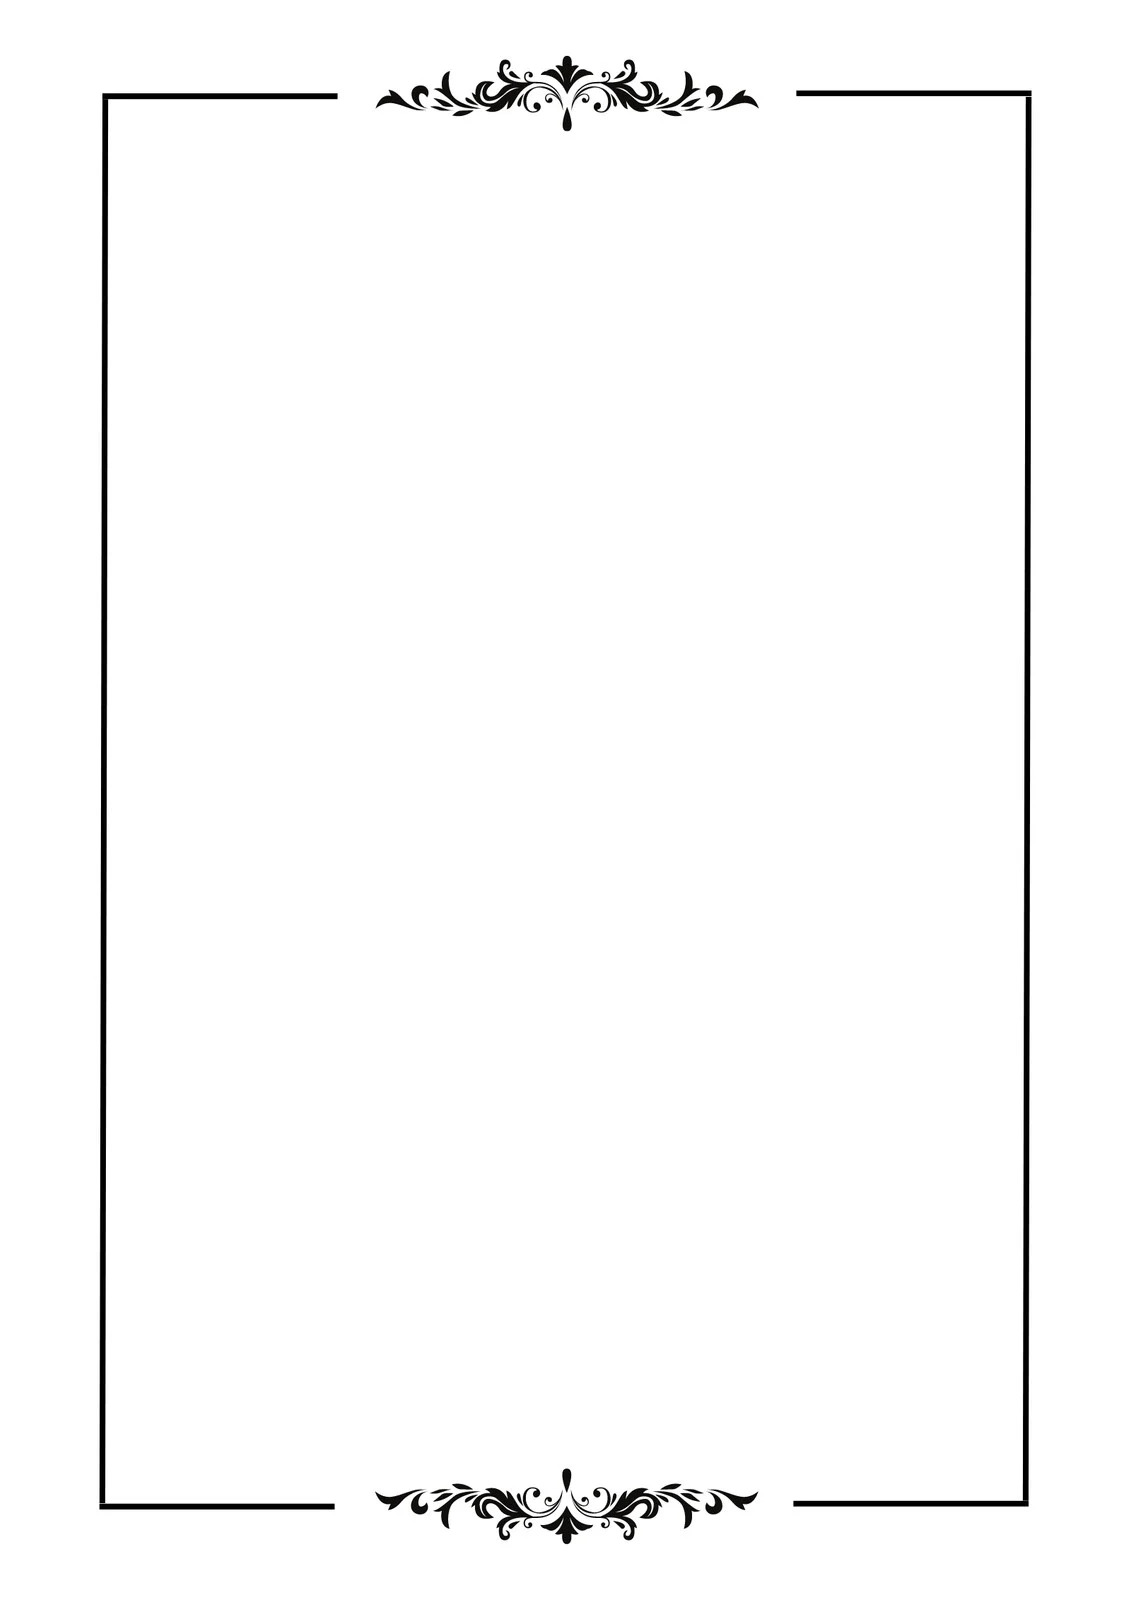
\includegraphics[width=\paperwidth,height=\paperheight]{./img/page-templates/leaves.jpg}
  }%
}


\pretitle{%
  \begin{center}
  \Large \textbf{ZÁKON HRY} \\ \Huge \textbf{Japanese Express} \\ \vspace{2.5cm}
  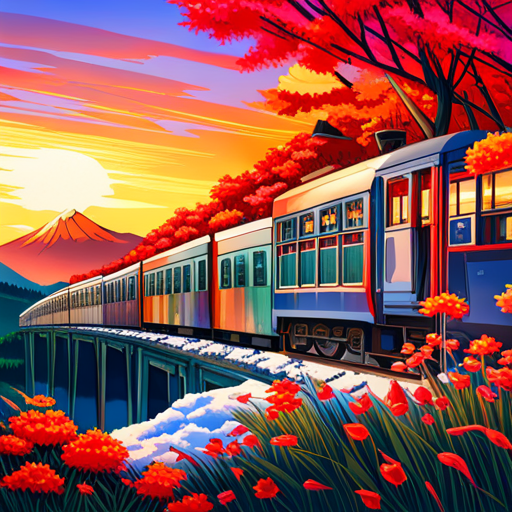
\includegraphics[width=7cm,height=7cm]{./img/logos/japanese-train4.png}\\[\bigskipamount] \vspace{2.5cm}
}
\posttitle{\end{center}}


\begin{document}
\BgThispage
\maketitle
\frenchspacing

\section{Základní informace}
\subsection{Herní prostor}

Hra se odehrává na středně velkém území v lese (celé území by mělo být na dohled). To se skládá de dvou částí: z výhybek rozmístěných po stromech a modelu aktuálně aktivních tratí.

\subsection{Hráči a týmy}

Hráči jsou rozděleni do 5 týmů podle svých družin.

\subsection{Struktura hry}

Hraje se na několik kol, přičemž každé kolo trvá zhurba 10 minut a skládá se ze dvou fází: \textit{\textbf{Přehození výhybek}} (6 min) a \textit{\textbf{Vyhodnocení}} (4 min). Všechny týmy hrají každou fázi současně.

\section{Dopravní plán}
\noindent Dopravní plán Japonské železniční dopravy se skládá z \textit{\textbf{výhybek}} a \textit{\textbf{tratí}}.

\subsection{Výhybky}
Každá výhybka má své jméno (např. "Chrám větru") a je možné ji nastavit do \textbf{jedné} ze sousedních výhybek. Sousední výhybka je vždy v plánu v pravo od ní a spojená čárou. Každá výhybka má 2 (např. "Rudá propast"), 3 nebo 5 sousedních výhybek. Poslední výhybky (např. "Malé prameny") je možné nastavit na libovolné území týmu. \\ Výhybky představují cedule rozvěšené po stromech. Červená rafička ukazuje která trať je právě aktivní. Rozmístění cedulí zhruba odpovídá rozmístění v plánu.

\subsection{Tratě}
Trať je cesta mezi výhybkami. Je znázorněná pouze v plánu a modelu tratí.

\section{Přehazování výhybek}
\noindent V každém kole se na začátku odehraje fáze Přehazování výhybek.

\subsection{Odpočítávání}
Hráči jsou v průběhu fáze, po určitých časových intervalech, informováni o zbývajícím čase. Až čas vyprší, bude nahlas oznámen konec fáze.

\subsection{Pohyb}
Dokud čas nevypršel, mohou se hráči volně pohybovat mezi výhybkami. Je ovšem zakázáno jakkoliv bránit jiným hráčům v pohybu. Ve chvíli, kdy je oznámen konec fáze, musí všichni zůstat stát na místě.

\subsection{Změna směru výhybky}
Na konci první fáze můžete přehodit směr výhybky ve vaší bezprostřední blízkosti. Směr změníte posunutím rafičky na ceduli. Pakliže se u jedné výhybky nachází více hráčů, sečtou se útočná čísla dohromady za celý tým. Tým s nejvyšším hromadným číslem si může vybrat kam výhybku přehodí. Pokud by nastala remíza (hromadná čísla jsou stejná) zůstává nastavení výhybku nepozměněné. \textit{\textbf{Útočné číslo}} každého hráče je \textbf{1 + jednotky samurajů} (4.4). Síla jednotek samurajů hráče není veřejná informace a nemusí jí nikomu zdělovat (naopak může blafovat).

\section{Vyhodnocení}
\subsection{Oznámení přehození výhybky}
Každý hráč, který přehodil některou z výhybek, dojde oznámit svou akci osobě u modelu aktivních tratí.
\subsection{Výjezd vlaků}
Po aktualizování modelu vyjede z každého japonského města jeden vlak. Tým, jemuž patří uzemí kam  dojede, získá \textbf{100 bodů}. Za jedno kolo je tedy možné získat až 400 bodů.

\subsection{Vítězství}
Hra končí v momentě, kdy některý z týmů získá více než \textbf{1400 bodů}. Tento tým okamžitě vyhrává.

\subsection{Jednotky samurajů}
Na konci fáze Vyhodnocení bude každému týmu přidělen stejný počet jednotek samurajů. Jednotky se mohou lišit v síle a není předem známo, jaké tým obdrží. Různé týmy mohou mít různě silné jednotky. Jednotky z předešlého kola naopak vrátí. Každý hráč smí mít u sebe pouze jednu jednotku. Jednotky je možné si vyměňovat pouze v rámci týmu a ve fázi Vyhodnocení.

\end{document}